\chapter{Numerical Time Integration of Partial/Ordinary Differential Equations}

\section{Introduction}

Many engineering problems are described as either a partial differential equation (PDE) or ordinary differential equation (ODE). A broad class of important problems is called the ``Initial Value Problem'' (IVP). Take for example the continuity equation in semiconductors, which is given as\begin{IEEEeqnarray}{rCl}
\frac{\partial n}{\partial t} & = & -\text{div}\left(\bm{J}\right) + G_\text{n} - R_\text{n} \label{eq:continuityEqn}
\end{IEEEeqnarray}where $n$ is the carrier concentration, $\bm{J}$ is the current density flowing through the semiconductor, $G_\text{n}$ and $R_\text{n}$ are the rates of carrier generation and recombination due to generation and recombination processes, respectively. The IVP would be as follows: assume that at time, $t=0$, the carrier concentration is $n(t=0)={0}$ and we want to find the time-dependent profile of the carrier concentration, $n(t)$.

In general, the PDE is more complicated than that in Equation~(\ref{eq:continuityEqn}), and the time derivative or slope function is denoted as $\dot{y}(t)=f(t, y)$, where $y(t)$ is the quantity we are trying to solve for, having the initial condition $y(t=0)=y_{0}$.

\section{The Forward (Explicit) Euler Method}

One method to obtain $y(t)$ from $f(t,y)$ and $y_{0}$ is to use the forward Euler method. First, the time range over which to determine $y(t)$ is discretized into a uniform grid. The time difference between each grid point, $\Delta t=h$ is called the \emph{time step}. $y(t)$ is then iteratively calculated (starting at $y_{0}$) using the formula\begin{IEEEeqnarray}{rCl}
y(t+h) & = & y(t) + hf(t,y(t)) \label{eq:compExEuler}
\end{IEEEeqnarray}Mathematically, the Equation~(\ref{eq:compExEuler}) is unwieldy and we simplify the expression using $y_{n+1}=y(t+h)$ and $y_{n}=y(t)$, which gives\begin{IEEEeqnarray}{rCl}
y_{n+1} & = & y_{n} + hf(t,y_{n}) \label{eq:simpExEuler}
\end{IEEEeqnarray}

\subsection{Example 1: Solutions with Persistent Oscillations}

Consider the function $y(t) = \sin (t)$ and its time derivative, $\dot{y}(t) = \cos (t)$. The numerical solution for different time steps are plotted in Fig.~\ref{fig:IVP1}. As clearly seen, the error reduces with the size of the time step---a smaller time step returns a numerical result that is closer to the ideal solution.

\subsection{Example 2: Solutions with Damped Relaxations}

Another commonly observed function is $y(t) = \exp(-t)$ and its time derivative, $\dot{y}(t) = -\exp(-t)$. The numerical solution for different time steps are plotted in Fig.~\ref{fig:IVP2}. As clearly seen, the error also reduces with the size of the time step.\afterpage{
\begin{figure}[!t]
\centering
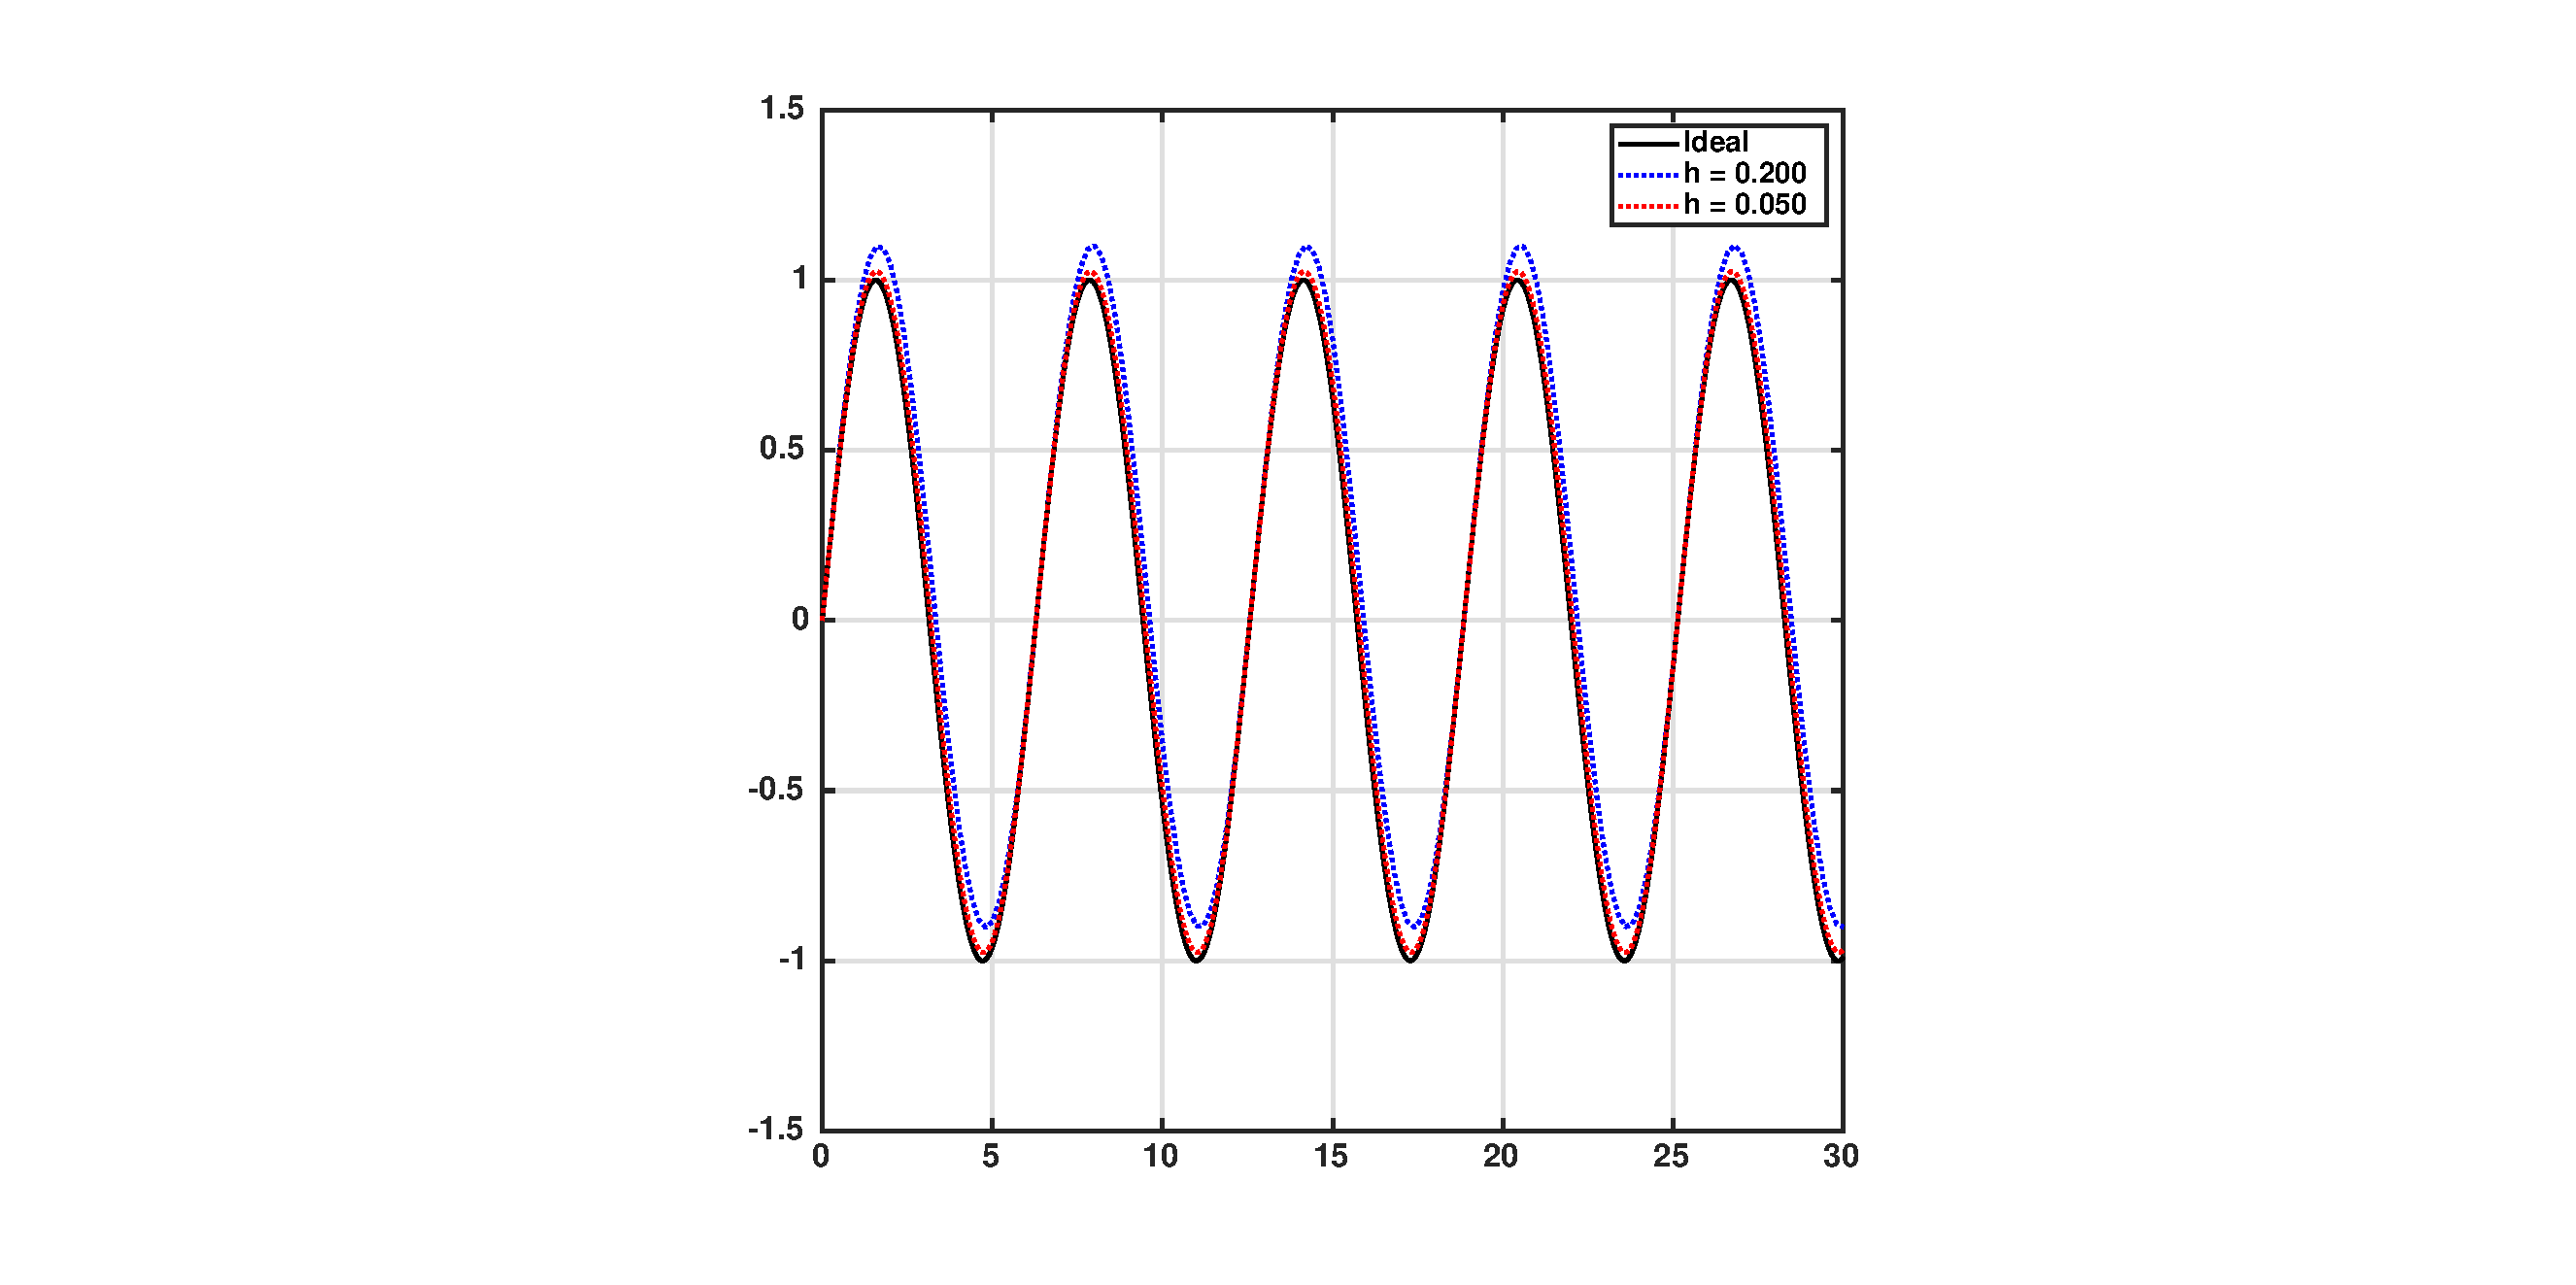
\includegraphics[scale=0.4]{ResearchNotes_TimePDE/figs/eulerTest.eps}
\caption{Numerical solution for the IVP with $\dot{y}(t)=\cos(t)$ and $y_{0}=0$ for different step sizes as compared to the ideal solution $y(t)=\sin(t)$.}
\label{fig:IVP1}
\end{figure}\begin{figure}[!t]
\centering
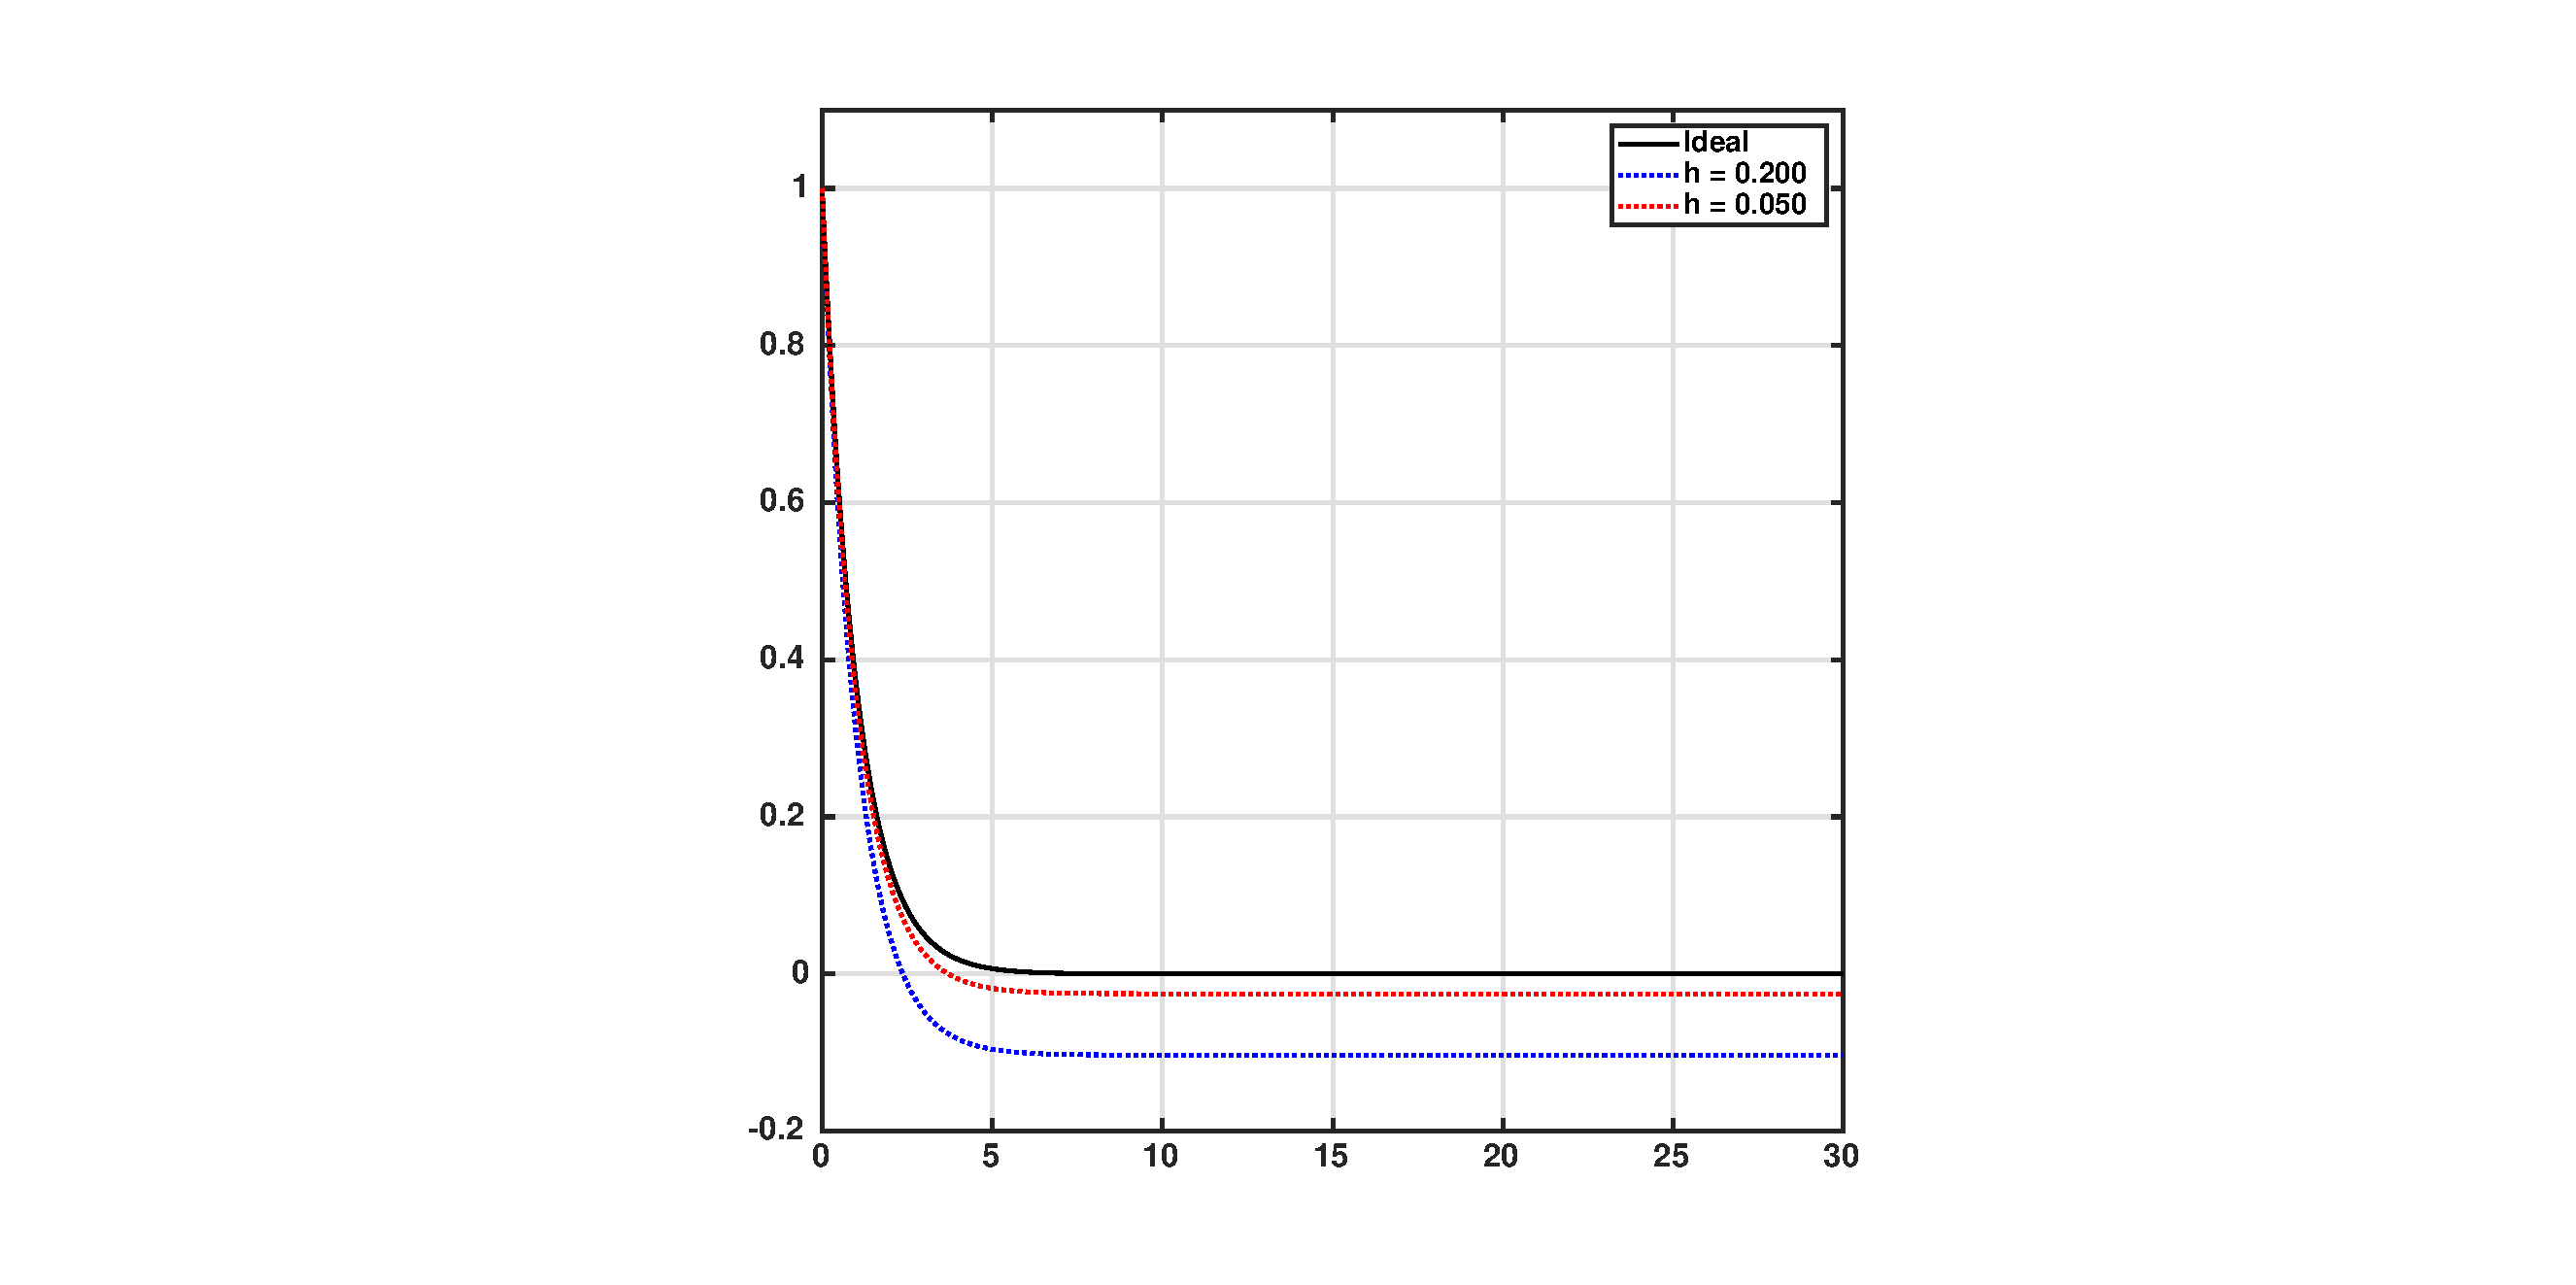
\includegraphics[scale=0.4]{ResearchNotes_TimePDE/figs/eulerTest2.eps}
\caption{Numerical solution for the IVP with $\dot{y}(t)=-\exp(-t)$ and $y_{0}=1.0$ for different step sizes as compared to the ideal solution $y(t)=\exp(-t)$.}
\label{fig:IVP2}
\end{figure}\clearpage
}

\section{Higher Order Explicit Methods}

Equation~(\ref{eq:simpExEuler}) has a similar form as the power series expansion, which is written as\begin{IEEEeqnarray}{rCl}
y(t) & = & \sum^{+\infty}_{n=0}a_{n}y^{(n)}(t)
\end{IEEEeqnarray}where the superscript $(n)$ denotes the $n$-th derivative of $y$. Thus, the forward Euler method may be thought of as a first order estimation for $y(t)$ and the full expression is\begin{IEEEeqnarray}{rCl}
y_{n+1} & = & y_{n} + hf(t,y_{n}) + \mathcal{O}(h^{2})
\end{IEEEeqnarray}and the error in using Equation~(\ref{eq:simpExEuler}) to approximate $y(t)$ is $\mathcal{O}(h^{2})$. By expanding the power series further, we can derive higher order explicit methods for $y_{n+1}$ and reduce the error.

\subsection{The Heun Method}

The Heun method is a second order method to approximate $y_{n+1}$ and is given by the expression\begin{IEEEeqnarray}{rCl}
y_{n+1} & = & y_{n} + h\frac{k_{1}+k_{2}}{2},~\text{where} \label{eq:heun} \\
k_{1} & = & f(t,y_{n}) \nonumber \\
k_{2} & = & f(t+h,y_{n}+hk_{1}) \nonumber
\end{IEEEeqnarray}It can be seen that $y_{n+1}$ is determined using two evaluations of $f()$ ($k_{1}$ and $k_{2}$). The evaluation of $k_{1}$ is akin to the explicit Euler method. The evaluation of $k_{2}$ occurs at the point predicted using the Euler method. The average of $k_{1}$ and $k_{2}$ is then used to estimate $y_{n+1}$.

\subsection{The 4-th Order Runge-Kutta (RK) Method}

German mathematicians Carl Runge and Wilhelm Kutta derived methods (also called Runge-Kutta methods or RK methods) to approximate $y_{n+1}$. The 4-th order RK method (RK4) is given by the expression\begin{IEEEeqnarray}{rCl}
y_{n+1} & = & y_{n} + \frac{h}{6}\left(k_{1}+2k_{2}+2k_{3}+k_{4}\right),~\text{where} \\
k_{1} & = & f(t,y_{n}) \nonumber \\
k_{2} & = & f\left(t+\frac{h}{2}, y_{n}+h\frac{k_{1}}{2}\right) \nonumber \\
k_{3} & = & f\left(t+\frac{h}{2}, y_{n}+h\frac{k_{2}}{2}\right) \nonumber \\
k_{4} & = & f(t+h,y_{n}+hk_{3}) \nonumber
\end{IEEEeqnarray}In this method $f()$ are evaluated at points within the time step to obtain a better approximation of $y_{n+1}$.

\subsection{The Butcher Tableau}

From the methods discussed so far, it can be seen that the general equation for determining $y_{n+1}$ is \begin{IEEEeqnarray}{rCl}
y_{n+1} & = & y_{n} + h\sum^{s}_{i=1}b_{i}k_{i},~\text{where} \\
k_{1} & = & f(t,y_{n}) \nonumber \\
k_{2} & = & f(t+c_{2}h,y_{n}+a_{21}k_{1}) \nonumber \\
k_{3} & = & f(t+c_{3}h,y_{n}+a_{31}k_{1}+a_{32}k_{2}) \nonumber \\
& \vdots & \\
k_{s} & = & f(t+c_{s}h, y_{n}+\sum^{s-1}_{j=1}a_{s,j}k_{j}) \nonumber
\end{IEEEeqnarray}The mathematician proposed a concise way of describing the numerical method for solving PDEs and ODEs using a tableau called the \emph{Butcher tableau} (see Fig.~\ref{fig:butcherTab}).

\begin{figure}[H]
\centering
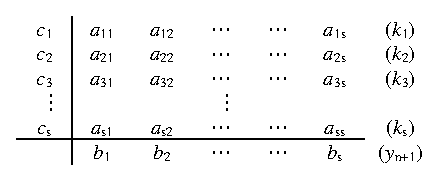
\includegraphics[scale=1.0]{ResearchNotes_TimePDE/figs/ButcherTableau.eps}
\caption{The general form of a Butcher Tableau}
\label{fig:butcherTab}
\end{figure}

From the earlier examples, we can see that the Butcher tableaus for the Euler method and RK4 method are given by Figs.~\ref{fig:eulerButcher} and Fig.~\ref{fig:rk4Butcher}. The Heun method is a special case of a more general method called the \emph{midpoint method}, which has the Butcher tableau given in Fig.~\ref{fig:midpointButcher}.

\begin{figure}[!b]
\centering

\includegraphics[scale=1.0]{ResearchNotes_TimePDE/figs/eulerButcher.eps}
\caption{Butcher Tableau for the Euler method.}
\label{fig:eulerButcher}
\end{figure}\begin{figure}[!b]
\centering
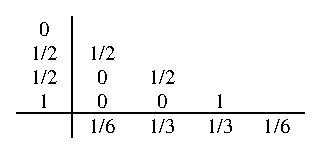
\includegraphics[scale=1.0]{ResearchNotes_TimePDE/figs/rk4Butcher.eps}
\caption{Butcher Tableau for the RK4 method.}
\label{fig:rk4Butcher}
\end{figure}\begin{figure}[!b]
\centering
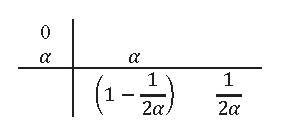
\includegraphics[scale=1.0]{ResearchNotes_TimePDE/figs/midpointTableau.eps}
\caption{Butcher Tableau for the midpoint method. The Heun method is the case where $\alpha=1$.}
\label{fig:midpointButcher}
\end{figure}

\section{Adaptive time stepping}

As can be seen in Figs.~\ref{fig:IVP1} and \ref{fig:IVP2}, there is a dependence of the accuracy of the solution returned by the numerical method and the time step used. In engineering simulations, the simulation runtime may be reduced is the time steps can be optimized. Adaptive time stepping algorithms attempt to optimize the time step used by ensuring that the estimated local truncation error (\emph{lte}) is bounded to some tolerance value. The lte is calculated by subtracting two approximations of $y_{n+1}$--one with order $p$ and another with order $p-1$, which leads to the lte having order $p$. These methods are sometimes called \emph{predictor-corrector} methods, since one expression gives a predicted value of $y_{n+1}$ and the lte gives a corrector t the predicted value.

A family of embedded RK methods exist that is computationally efficient in calculating $y_{n+1}$ and the lte, $\widehat{\bm{e}}$. These methods are computationally efficient because they reduce the number of calls to evaluate $f()$, which is the most computationally intensive portion of the numerical method. Fig.~\ref{fig:embeddedButcher} shows the general form of the Butcher tableau for an embedded method.

\begin{figure}[H]
\centering
\begin{minipage}{0.45\linewidth}
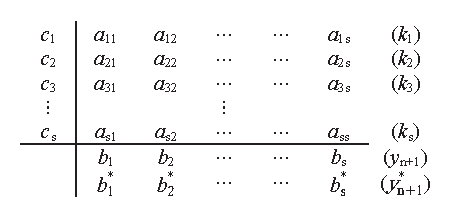
\includegraphics[scale=1.0]{ResearchNotes_TimePDE/figs/EmbeddedButcherTableau.eps}
\caption{The general Butcher tableau for embedded methods.}
\label{fig:embeddedButcher}
\end{minipage}
\quad\quad
\begin{minipage}{0.45\linewidth}
\centering
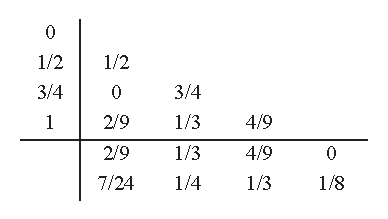
\includegraphics[scale=0.8]{ResearchNotes_TimePDE/figs/rk23.eps}
\caption{The Butcher tableau for the Bogacki-Shampine method. The method has a second order predictor and third order corrector and the lte is $\bm{O}(h^{3})$.}
\label{fig:rk23}
\end{minipage}
\end{figure}

Some commonly used embedded explicit methods are those by Bogacki-Shampine (RK23) \cite{Bogacki1989}, Fehlberg (RK45F) \cite{Fehlberg1970}, Cash-Karp (RF45CK) \cite{Cash1990}, and Dormand-Prince (RK45DP) \cite{Dormand1980}. There are shown in Fig.~\ref{fig:rk23} to \ref{fig:rk45dp}. A key difference between the RK45 methods is the number of evaluations of $f()$ needed to estimate $y_{n+1}$.

\begin{figure}[H]
\centering
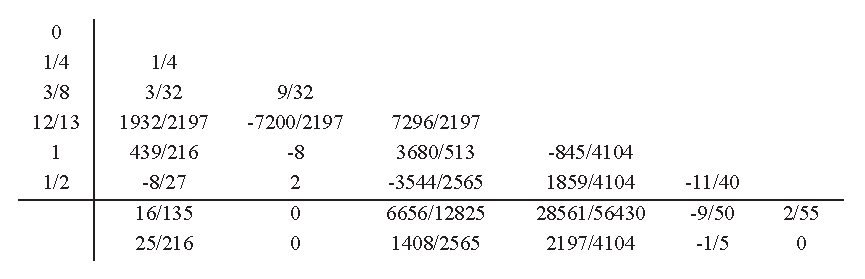
\includegraphics[scale=0.8]{ResearchNotes_TimePDE/figs/fehlberg.eps}
\caption{The Butcher tableau for the Fehlberg method. The method has a fourth order predictor and fifth order corrector and the lte is $\bm{O}(h^{5})$.}
\label{fig:fehlberg}
\end{figure}\begin{figure}[H]
\centering
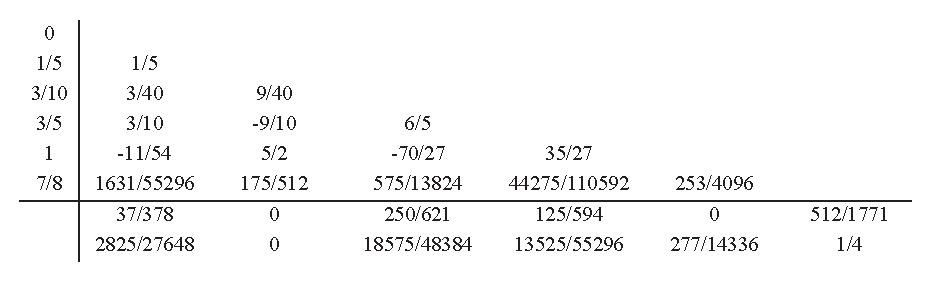
\includegraphics[scale=0.8]{ResearchNotes_TimePDE/figs/rk45ck.eps}
\caption{The Butcher tableau for the Cash-Karp method. The method has a fourth order predictor and fifth order corrector and the lte is $\bm{O}(h^{5})$.}
\label{fig:rk45ck}
\end{figure}\begin{figure}[H]
\centering
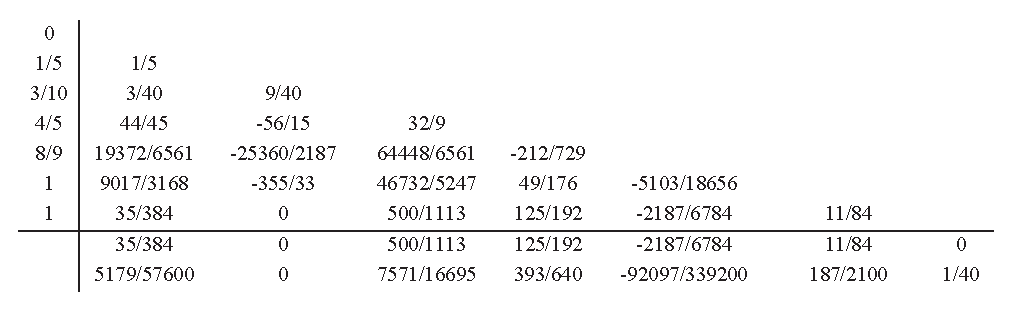
\includegraphics[scale=0.8]{ResearchNotes_TimePDE/figs/rk45dp.eps}
\caption{The Butcher tableau for the Dormand-Prince method. The method has a fourth order predictor and fifth order corrector and the lte is $\bm{O}(h^{5})$.}
\label{fig:rk45dp}
\end{figure}

Adaptive time stepping is performed by calculating the ratio of an error tolerance to the lte. The next time step in the numerical method is then scaled according to the equation\begin{IEEEeqnarray}{rCl}
h_{n+1} & = & 0.9 \times h_{n} \times \min\left(\max \left(\left(\frac{\text{tol}}{|\widehat{\bm{e}}|}\right)^{1/p},0.3\right), 2\right)
\end{IEEEeqnarray}where $p$ is the order of the corrector. The factor of 0.9 is a safety factor to limit the change in $h$. The $\min$ and $\max$ further limit $h_{n+1}$ to the range $[0.27h_{n}, 1.8h_{n}]$.

\subsection{Stability of Explicit Methods and Stiffness of IVP}

A major disadvantage of explicit methods is that the errors introduced when used to solve stiff IVPs can be extremely large. Examples of stiff problems are encountered when critically damped and overdamped systems are studied. Consider the example of a non-ideal voltage source charging a fixed capacitor, $C_\text{L}$, through an output resistance, $R_\text{out}$ to a voltage given by $V_\text{DD}$. The circuit equation to solve is the ODE expressed as\begin{IEEEeqnarray}{rCl}
\frac{d V_\text{C}}{dt} & = & \frac{V_\text{DD}-V_\text{C}}{R_\text{out}C_\text{L}}
\end{IEEEeqnarray}The ideal solution for the voltage across the capacitor, $V_\text{C}(t)$, when the initial condition is 0~V is\begin{IEEEeqnarray}{rCl}
V_\text{C}(t) & = & V_\text{DD}\left(1-\exp\left(\frac{-t}{R_\text{out}C_\text{L}}\right)\right)
\end{IEEEeqnarray}Fig.~\ref{fig:falseOscillation} shows a case where a poorly chosen time step leads to a numerical solution that continually oscillates without converging to the steady-state solution.

\begin{figure}[H]
\centering
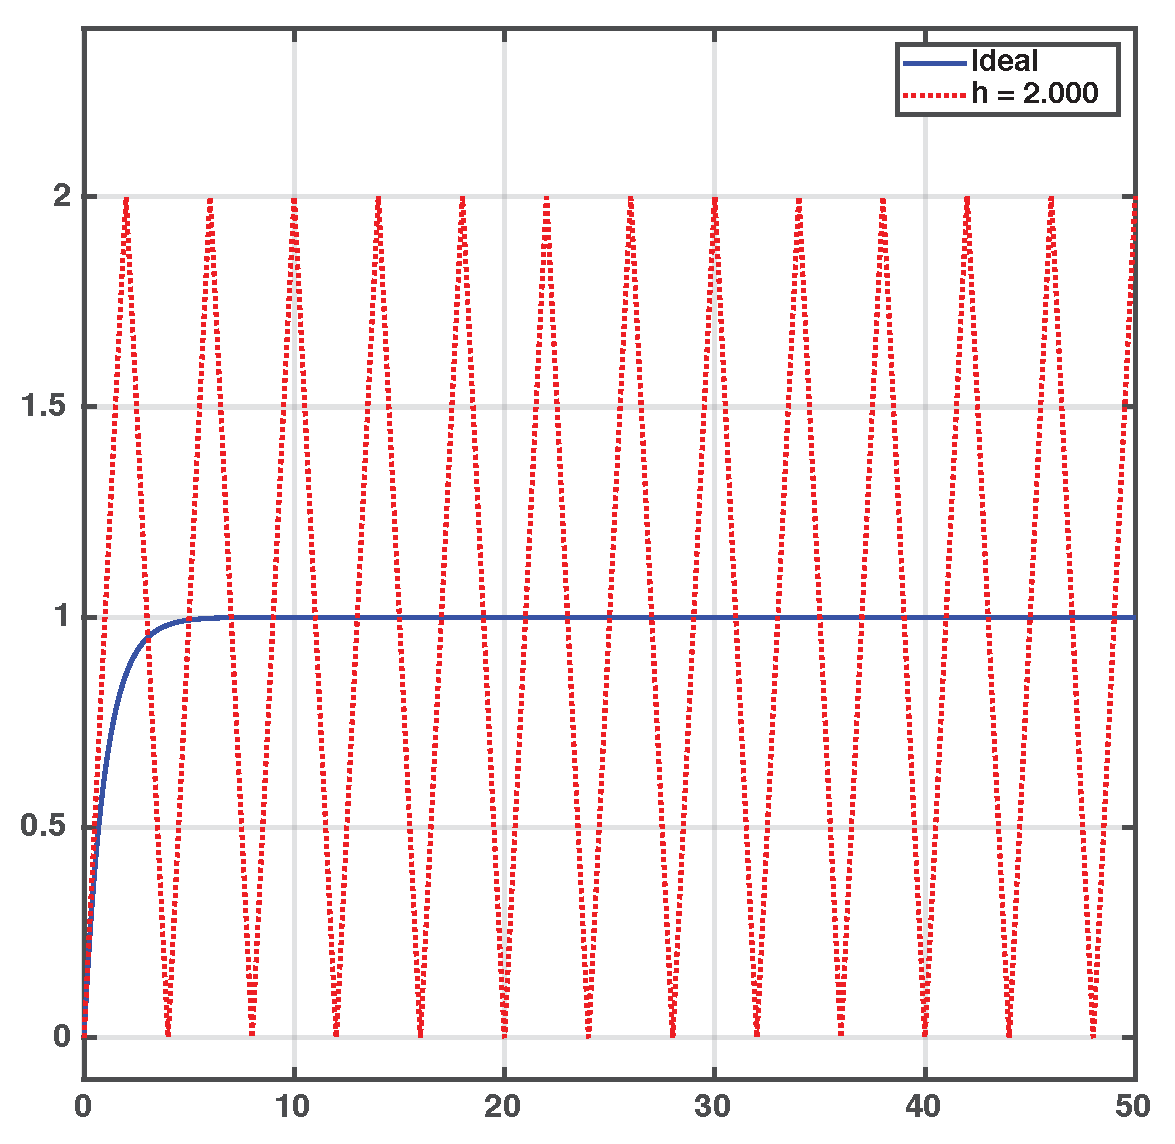
\includegraphics[scale=0.4]{ResearchNotes_TimePDE/figs/forwardOscillations.eps}
\caption{Poor numerical solution with oscillations was obtained as the problem is too stiff for the explicit numerical method.}
\label{fig:falseOscillation}
\end{figure}

\section{The Backward (Implicit) Euler Method}

